\section{Cross-Setting Transfer: Pythia Induction}\label{sec:pythia}

\subsection{Can the GPT-2 fine mechanism transfer?}\label{sec:pythia-design}

We test the GPT-2 target-positive/rival-negative pattern in a different model family and task: Pythia-160M on repeated-token induction. The transfer hypothesis was specified prospectively: after selecting a later head that becomes more useful when an earlier induction head is removed, FALI should again yield $\phi_T>0$ and $\phi_R<0$.

Head selection was separated from FALI attribution. Discovery used seed 42 only and did not inspect fine FALI attributions; the frozen selection procedure chose L5H0 as the primary head and L8H2 as the candidate. Confirmation used independent seeds 1, 8, and 22 across offsets 8, 16, and 24, with 128 examples per offset per seed. The repeated-token construction, matched control, sampling details, and bootstrap procedure are described in the Supplementary Information.

\subsection{Recruitment transfers; the fine mechanism does not}\label{sec:pythia-results}

The held-out cohorts satisfy the functional prerequisites. The induction advantage is $14.017$ (95\% CI $[12.280,15.939]$), removing L5H0 produces a primary drop of $1.146$ ($[0.887,1.539]$), and L8H2 is positively recruited: conditional effect $0.621$ ($[0.456,0.860]$) and conditional gain $0.486$ ($[0.326,0.722]$). Figure~\ref{fig:cross-setting-reversal}a therefore establishes the shared high-level phenomenon: positive conditional recruitment occurs in both the GPT-2 IOI and Pythia induction cases studied here.

The fine mechanism, however, reverses. For Pythia L8H2, FALI gives $\phi_T=-0.144$ (95\% CI $[-0.247,-0.084]$) and $\phi_R=+0.118$ ($[0.058,0.219]$), with the reversed signs in every confirmation seed and offset. The other score and value channels are small ($\phi_O=-0.00027$, $\phi_V=-0.00210$), while the surrounding-context contribution is positive and large ($\phi_C=0.514$). As elsewhere, $C$ denotes coarse surrounding computation rather than a uniquely localized mechanism.

Figure~\ref{fig:cross-setting-reversal}b places the two settings side by side: GPT-2 IOI recruitment is target-positive and rival-negative, whereas Pythia induction recruitment is target-negative and rival-positive. The preregistered mechanism-transfer hypothesis therefore fails. No alternate head pair, model, task, or threshold was substituted after observing this result.

The inference is intentionally bounded. The experiment shows that positive conditional recruitment can occur with opposite fine target/rival organizations under the specified FALI games. It does not establish that recruitment mechanisms are universally different across model families, nor that no deeper common mechanism exists. Because model, task, head pair, perturbation, and metric all change between the two settings, the experiment is a mechanism-discrimination test rather than a controlled explanation of which factor caused the reversal.

\begin{figure*}[t]
\centering
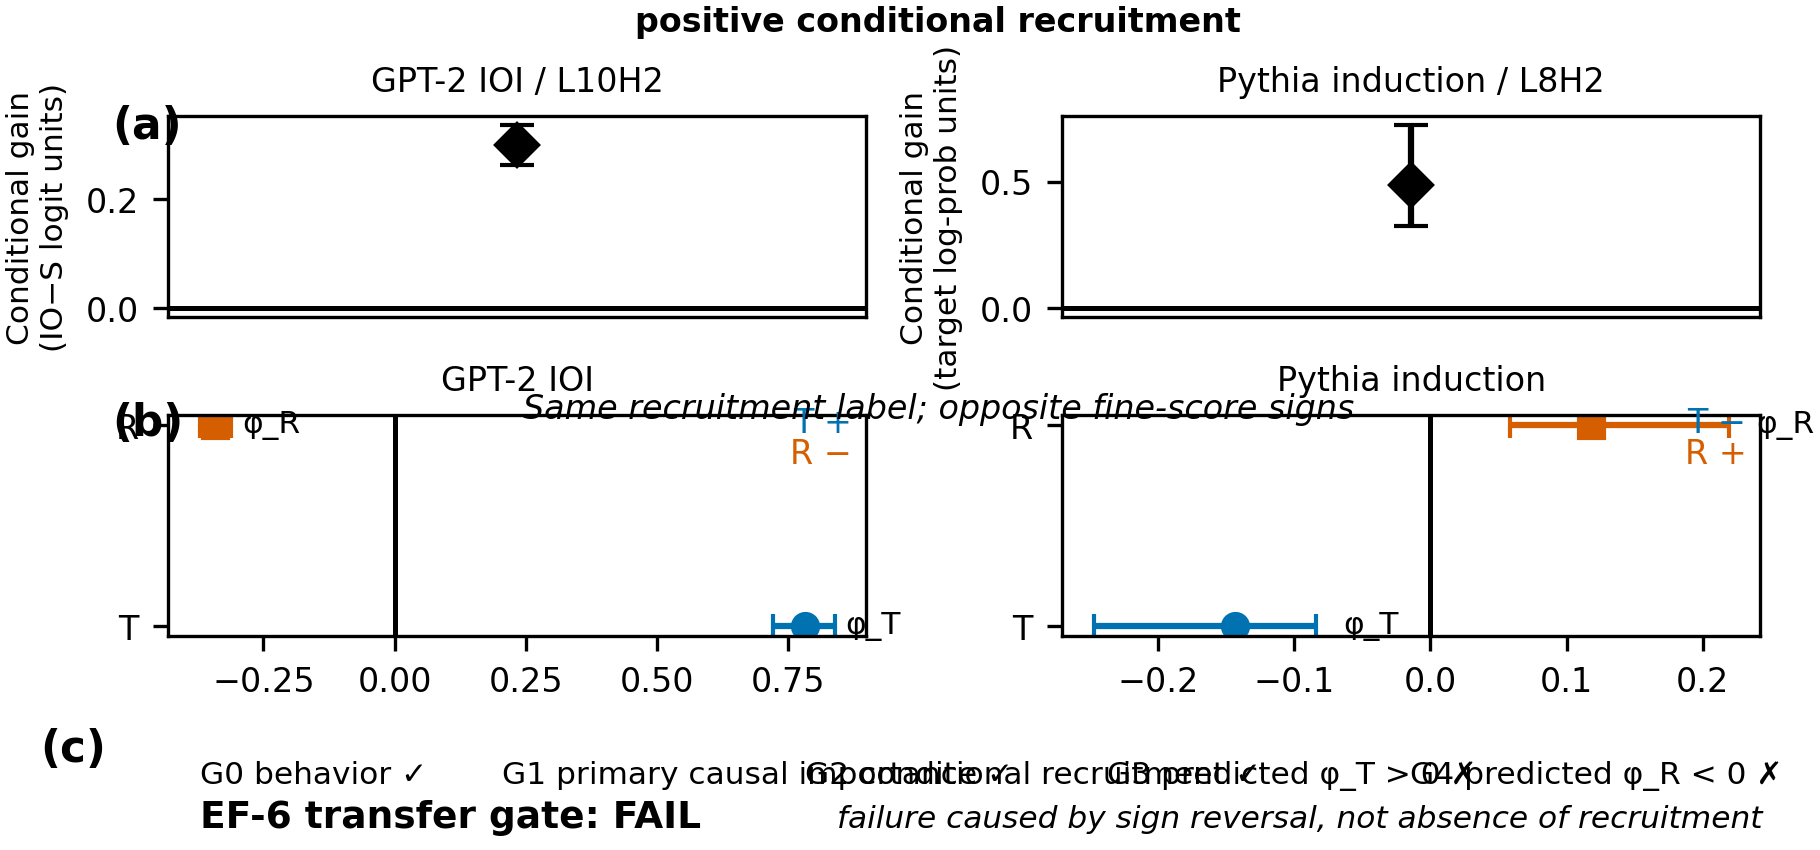
\includegraphics[width=\textwidth]{figures/Fig5.png}
\caption{\textbf{Conditional recruitment transfers across the two studied settings, but the preregistered fine-score mechanism does not.}
GPT-2 IOI L10H2 and Pythia-160M induction L8H2 both have positive conditional gain after their respective primary interventions; their raw attribution magnitudes are shown on task-specific utility scales and should not be compared directly.
Their fine FALI signs reverse: GPT-2 is target-positive/rival-negative with a negative context contribution, whereas Pythia is target-negative/rival-positive with a positive context contribution.
The preregistered Pythia transfer test therefore fails both sign-transfer gates while retaining confirmed induction behavior, primary-head importance, and conditional recruitment (G0--G2), giving an overall EF-6 transfer-gate failure.
Thus, a common functional recruitment response does not imply a common fine-grained mechanism.}
\label{fig:cross-setting-reversal}
\end{figure*}

